%%% --------------------------------------------------------
%%> \section{Директиви компілятора}
%%% --------------------------------------------------------

% !TeX program = lualatex
% !TeX encoding = utf8
% !BIB TS-program = biber




\documentclass[]{iptconf}





%%% --------------------------------------------------------
%%> \section{Реєстраційна форма}
%%% --------------------------------------------------------





\regform{
    fullname = {Аватар Великович Тор},          % Повне ім'я доповідача (перший автор)
    birthday = {01.02.1990},                    % Дата народження доповідача
    position = {асистент},                      % Посада доповідача
    phone = {+380935555555},                    % Телефонний номер доповідача
    authoremail = {mr_thor@gmail.com},          % Email доповідача
    confsection = {Фізика енергетичних систем}, % Секція конференції,
    copynum = {0},                              % Замовлена число друкованого збірника
    needliving = {ні},                          % Потреба в житлі (Ні/Хостел/Готель/інше)
    needinvitanion = {ні},                      % Чи потрібне запрошення на конференцію?
}





%%% --------------------------------------------------------
%%> \section{Використані пакети}
%%% --------------------------------------------------------





\usepackage[most]{tcolorbox}
\usepackage{tabularray}
\UseTblrLibrary{booktabs}
\usepackage{mathtools}
\usepackage{dsfont}
\usepackage{mathrsfs}
\usepackage{wrapfig}
\usepackage{xurl}
\usepackage[version=4]{mhchem}
\usepackage{forest}
\usepackage{tikz}
\usepackage{pgfplots}
\usepackage{listings}
\usetikzlibrary{shadows,arrows.meta}





%%% --------------------------------------------------------
%%> \section{Файл бібліографії}
%%% --------------------------------------------------------





%% Змініть ім'я файлу бібліографі на ваш.
%% Краще, щоб його назва була така ж сама,
%% як у вашого .tex-файлу

\addbibresource{template.bib}





%%% --------------------------------------------------------
%%> \section{Команди користувача}
%%% --------------------------------------------------------





\def\templateurl{%
\href{https://drive.google.com/file/d/1YrrTXnwaIcydBJLFS5BM6uj-yosnkRl3/view}%
{\texttt{author.zip}}}





%%% --------------------------------------------------------
%%> \section{Заголовок статті}
%%% --------------------------------------------------------





\title{Рецепти написання матеріалів \\ \NoCaseChange{\ce{Na2ZnO2.4H2O}}}





%%% --------------------------------------------------------
%%> \section{Автори}
%%% --------------------------------------------------------





%%Якщо бажаєте, введіть
% e-mail автора в квадратних дужках:
\author[email1@mail.com]{А.~В.~Перший}{1}
\author{А.~В.~Другий}{2}
\author{А.~В.~Третій}{2}

%% Якщо  автор працює в кількох установах,
%% то треба вводити номери установ через кому,
%% наприклад так:
\author[email3@mail.com]{А.~В.~Четвертий}{1,2}





%%% --------------------------------------------------------
%%> \section{Установи}
%%% --------------------------------------------------------





%% Тут введіть установув якій працює, або навчається перший автор.
%% Введіть \ipt якщо автор навчається, або працює в НТУУ "КПІ"
\affiliation{\ipt}{1}

%% Тут введіть установу в якій працює, або навчається другий автор
\affiliation{Установа, в якій працює, або навчається другий автор}{2}





%%% --------------------------------------------------------
%%> \section{УДК та PACS}
%%% --------------------------------------------------------





%\pacs{ }
\udc{501}





%%% --------------------------------------------------------
%%> \section{Анотація до статті}
%%% --------------------------------------------------------

\abstract{

    Ця стаття містить інформацію про те, як вам подати тези на нашу конференцію. Він був згенерований з \texttt{.tex}-файлу, який одночасно є шаблоном для оформлення матеріалів. В \texttt{.tex}-файлі також зібрані рецепти, які вам знадобляться для написання гарно оформлених матеріалів. Не нехтуйте ними.

    І пам'ятайте, якщо \texttt{MS Word} --- це швидко і аби-як, то \LaTeX --- це осмислено і гарно. Не відносьтесь до своїх матеріалів <<на відчепись>>, спробуйте вкласти в них <<душу>> як у зміст так і в оформлення.

}





%%% --------------------------------------------------------
%%> \section{Ключові слова}
%%% --------------------------------------------------------





\keywords{розділи, стаття, тези}




\begin{document}





%%% --------------------------------------------------------
%%> \section{Мова статті}
%%% --------------------------------------------------------





\PaperLanguage{ukrainian} %





%%% --------------------------------------------------------
\section*{Вступ}
%%% --------------------------------------------------------





Оформлення матеріалів конференції здійснюється у форматі \TeX. Про правила набору та верстки в системі \LaTeX{} можна дізнатись із книг \cite{Lvovsky} та \cite{Voron05latex}, які є у вільному доступі на теренах
\texttt{internet}'у, також  ви можете скористатись сайтом \href{http://tex.stackexchange.com/}{tex.stackexchange.com}, на якому можна як задавати питання, так і шукати необхідні відповіді.





%%% --------------------------------------------------------
\section{Надсилання матеріалів}
%%% --------------------------------------------------------




%%% --------------------------------------------------------
\subsubsection*{Що і куди Ви повинні надіслати...}
%%% --------------------------------------------------------





\begin{tcolorbox}[breakable,enhanced,arc=0mm,colback=gray!5,colframe=red!80!black,leftrule=2mm]
	%	Зареєструйтесь як автор на сайті \url{conference.ipt.kpi.ua} і надішліть матеріали у вигляді zip-архіву, який буде мати такий вигляд: \par\textcolor{red}{ <<ім'я першого автора статті латиницею>>.zip}
	Надішліть матеріали у вигляді zip-архіву, який буде мати такий вигляд:

	\medskip

	\textcolor{red}{ <<ім'я першого автора статті латиницею>>.zip}

	\medskip

	на електронну адресу відповідної секції. Електронні скриньки секцій ви можете знайти на сайті конференції  \url{http://conf.ipt.kpi.ua}.
\end{tcolorbox}

%Якщо Вас виникають проблеми з реєстрацією на сайті \url{conference.ipt.kpi.ua}, радимо прочитати  \href{https://drive.google.com/file/d/0B3_rN9Ji08-VVk9nWW5KNE5PcnM/view}{інструкцію по реєстрації}.





%%% --------------------------------------------------------
\subsubsection*{Де взяти шаблон оформлення...}
%%% --------------------------------------------------------





Шаблон міститься в архіві \templateurl, який можна завантажити на сайті конференції.

%Файл \texttt{author.tex} -- є прикладом і одночасно шаблоном для оформлення тез конференції.

Після його завантаження
\begin{tcolorbox}[breakable,enhanced,arc=0mm,colback=gray!5,colframe=red!80!black,leftrule=2mm]
	обов'язково перейменуйте файл \texttt{author.tex}.
\end{tcolorbox}

Назва \texttt{.tex}-файлу повинна йменуватись прізвищем першого автора тез латиницею і мати ту ж саму назву, що і тека в якій він лежить.

Наприклад \texttt{\textbackslash Kuzmenko\textbackslash Kuzmenko.tex}.





%%% --------------------------------------------------------
\subsubsection*{Що повинно міститись в \texttt{zip}-архіві...}
%%% --------------------------------------------------------

Після того, як ви вдало скомпілюєте файл, ваша тека має містити файли на зразок наведених нижче:

\begin{tcolorbox}[boxrule=0mm, sharpish  corners]
	\texttt{d:\string\Kuzmenko}\\
	\texttt{..}\\
	\texttt{iptconf.cls}\\
	\texttt{image.png}\\
	\texttt{Kuzmenko.aux}\\
	\texttt{Kuzmenko.dat}\\
	\texttt{Kuzmenko.log}\\
	\texttt{Kuzmenko.out}\\
	\texttt{Kuzmenko.pdf}\\
	\texttt{\textcolor{red}{Kuzmenko.tex}}\\
	\texttt{Kuzmenko.bib}
\end{tcolorbox}

Заархівуйте цю теку архіватором \texttt{zip} і надішліть її на адресу відповідної секції. Інформація про секції на сайті \url{conf.ipt.kpi.ua}.





%%% --------------------------------------------------------
\section{Способи компіляції \texttt{.tex}-файлу}
%%% --------------------------------------------------------





Неважливо, який із способів компіляції, з наведених нижче ви оберете, важливо дотриматись наступних вимог:
\begin{tcolorbox}[breakable,enhanced,arc=0mm,colback=gray!5,colframe=red!80!black,leftrule=2mm]
	\begin{itemize}
		\item Компілювати необхідно за допомогою драйверу \textcolor{red}{\textbf{\texttt{lualatex.exe}}},
		\item Кодування \texttt{author.tex}-файлу  має бути \textcolor{red}{\textbf{\texttt{utf8}}},
		\item Файл \texttt{ConfFTI.cls}, має міститись в тій же теці, що і ваш файл \texttt{.tex}-файл.
	\end{itemize}
\end{tcolorbox}





%%% --------------------------------------------------------
\subsection{Компіляція на домашньому ПК}
%%% --------------------------------------------------------





Для компіляції \texttt{.tex}-файлу на домашньому ПК, вам знадобиться встановити один із дистрибутивів \TeX. Для \texttt{ОС Windows} є два найбільш поширених на сьогодні дистрибутиви, \href{http://miktex.org/}{Mik\TeX} та \href{https://www.tug.org/texlive/}{\TeX live}. Можете вільно завантажити якийсь із них, та встановити на своєму ПК.

Для зручної роботи з \texttt{.tex}-файлами можна встановити один з редакторів (\href{http://texstudio.sourceforge.net/}{\TeX studio}, \href{http://www.winedt.com/download.html}{WinEdt}, \href{https://www.tug.org/texworks/}{\TeX Works} тощо).

Ви маєте користуватись даним шаблоном, в якому присутні усі основні конструкції, що можуть стати у нагоді, необхідно лише знайти необхідний шматок у \texttt{.tex}-файлі і заповнити його потрібною інформацією.





%%% --------------------------------------------------------
\subsection{Компіляція online}
%%% --------------------------------------------------------

Якщо ви не бажаєте встановлювати будь-який дистрибутив \TeX{} на свій комп'ютер, то є
можливість зробити це через \texttt{internet} за допомогою сервісу	 \href{https://www.overleaf.com/}{\texttt{www.overleaf.com}}.

Приклад проекту, створеного з файлів шаблону  цієї конференції \templateurl{} можна знайти за цим посиланням   \url{https://overleaf.com/read/tmhxcthgrzcm}.

Створіть свій особистий проект та назвіть його прізвищем першого автора латиницею.

Завантажте в теку проекту файли з архіву \templateurl.

В вашому проекті обов'язково мають бути файли
\begin{itemize}
	\item файл \texttt{iptconf.cls};
	\item файл \texttt{author.tex} (перейменуйте його прізвищем першого автора латиницею);
	\item файл \texttt{author.bib} (в разі, якщо ви ним користуєтесь, перейменуйте його також прізвищем першого автора латиницею);
	\item файли ваших зображень.
\end{itemize}

\begin{tcolorbox}[breakable,enhanced,arc=0mm,colback=gray!5,colframe=red!80!black,leftrule=2mm]
	Після компіляції обов'язково перегляньте логи на предмет можливих помилок і створений \texttt{pdf}-файл,
\end{tcolorbox}

\noindent якщо його вигляд вас влаштовує,

\begin{tcolorbox}[breakable,enhanced,arc=0mm,colback=gray!5,colframe=red!80!black,leftrule=2mm]
	завантажте свій проект (\texttt{.tex}, \texttt{.cls}, файли зображень) разом зі згенерованими сервісом файлами (\texttt{.pdf}, \texttt{.bbl}, \texttt{.dat}). Помістіть ці файли в папку (назва як і \texttt{.tex}-файл), заархівуйте і надішліть на пошту відповідної секції (\url{http://conf.ipt.kpi.ua/?p=10}).
\end{tcolorbox}

Файли \texttt{.bbl} і \texttt{.dat} можна знайти в кінці списку логів (див. пояснення  \href{https://www.overleaf.com/help/207-how-do-i-download-the-aux-and-the-bbl-files-my-publisher-asked-me-to-include-them-in-my-submission#.VvMwEnpCh2M}{overleaf}).





%%% --------------------------------------------------------
\subsection{<<Правила етикету>> при наборі тез в \LaTeX}
%%% --------------------------------------------------------





Для того,щоб ваші матеріали виглядали найкращим чином, при їх оформленні, слід дотримуватись певних <<правил етикету>>:

\begin{enumerate}
	\item Тире <<-->> слід ставити у вигляді подвійного знака мінус, наприклад:

	      \verb|Тире~--- це знак|.

	      Знак <<\verb|~|>> означає нерозривний пробіл, а <<\verb|---|>> створить тире необхідної довжини.

	\item Для лапкок, слід використовувати подвійні знаки менше-більше \verb|<< >>|, наприклад:
	      \begin{verbatim}
     <<Наразі в українській мові,
     не існує єдиного загальноприйнятого
     варіанту лапок>>.
     \end{verbatim}

	\item Всі цифри і латинські позначення для математичних величин в тексті, слід оточувати одинарними знаками долару, наприклад:
	      \verb|$0$~років тому|,

	      Електричний опір \verb|$R$|,

	      Величина \verb|$X$ становить$~\% від загальної|

	\item Величини з розмірностями, що набрані безпосередньо в рядку слід оточувати одинарними знаками долару, кириличні найменування величин слід записувати в тезі \string\text, наприклад:
	      Енергія активації хімічної реакції \verb|$E=300\text{кДж/моль}$|

	      \verb|Температура $T=30^\circ C$|

	\item Посилання на літературу, рисунки, формули та таблиці повинні мати вигляд:
	      \verb|На рис.~\ref{pic1}|

	      \verb|В таблиці~\ref{tab1}|

	      \verb|Згідно формули \eqref{eq}|

	      \verb|В роботах~\cite{robota1, robota2} показано|
\end{enumerate}





%%% --------------------------------------------------------
\section{Найбільш вживані конструкції \LaTeX}
%%% --------------------------------------------------------





%%% --------------------------------------------------------
\subsection{Списки та переліки}
%%% --------------------------------------------------------





Для верстки тексту тез слід, де це можливо, використовувати \emph{нумеровані} або
\emph{марковані} списки. Списки, як і таблиці, допомагають структурувати матеріал.
\begin{enumerate}
	\item Приклад нумерованого списку.
	\item Списки з глибиною вкладеності більше двох-трьох рівнів використовувати не рекомендується.
\end{enumerate}

\begin{itemize}
	\item Приклад маркованого списку.
	      \begin{itemize}
		      \item Елемент другого рівня.
	      \end{itemize}
\end{itemize}

\begin{enumerate}
	\item Нумеровані та марковані списки можна змішувати
	      \begin{itemize}
		      \item в різних комбінаціях.
	      \end{itemize}
\end{enumerate}





%%% --------------------------------------------------------
\subsection{Математичні формули в \LaTeX}
%%% --------------------------------------------------------





Математичні формули в \LaTeX{} можна набирати в двох режимах: у тексті абзацу і між абзацами.
Приклад математичних формул в тексті: $x \in X$, $X = \{\alpha, \beta, \gamma, \dots,
	\omega\}$; $(a \le b) \wedge (b \le c) \Rightarrow a \le c$. Для набору математичних формул
між абзацами тексту існує кілька видів спеціальних середовищ (див. документацію до пакету
\href{http://mirror.ctan.org/macros/latex/required/amslatex/math/amsldoc.pdf}{\texttt{amsmath}}.

Для верстки одиничних рівнянь \textit{з нумерацію} використовується оточення \texttt{equation}:
\begin{equation}
	\label{eq:Diskriminant} %% Це мітка на рівняння,
	%% посилатись на нього треба як \eqref{eq:Diskriminant}
	D = \sqrt {{b^2} - 4ac}
\end{equation}

Для верстки одиничних рівнянь \textit{без нумерації} використовується оточення \texttt{equation*}
(з зірочкою):
\begin{equation*}
	D = \sqrt {{b^2} - 4ac}
\end{equation*}

Для верстки декількох формул поспіль можна використовувати оточення \texttt{gather}
\begin{gather}
	(a+b)^3 = a^3 + 3a^2b + 3ab^2 + b^3,\\
	(a+b+c)^2 = a^2 + b^2 + c^2 +\nonumber\\
	+ 2ab + 2ac + 2bc.
\end{gather}
або \texttt{align}:
\begin{align}\label{eq:aligned_equation}
	(a+b)^3   & = a^3 + 3a^2b + 3ab^2 + b^3,        \\
	(a+b+c)^2 & = a^2 + b^2 + c^2 + 2ab + \nonumber \\
	          & + 2ac + 2bc.
\end{align}

Для верстки довгих формул, які не поміщаються в одному рядку, можна використовувати
оточення \texttt{multlin} додавши \texttt{\string\\} в місці розриву:

\begin{multline}\label{eq:multined_equation}
	(a+b+c)^2 + (d+e+f)^2 + (g+h+i)^2 = \\
	= a^2 + b^2 + c^2 + 2ab + 2ac + 2bc +\\
	+d^2 + e^2 + f^2 + 2de + 2df + 2ef +\\
	+g^2 + h^2 + i^2 + 2gh + 2gi + 2hi.
\end{multline}

%Для посилання на розмічені за допомогою міток \string\label\ рівняння, можна посилатись за допомогою команди \string\eqref, наприклад \eqref{eq:Diskriminant}, \eqref{eq:aligned_equation}, \eqref{eq:multined_equation}.

\begin{tcolorbox}[breakable,enhanced,arc=0mm,colback=gray!5,colframe=red!80!black,leftrule=2mm]
	Якщо збираєтесь посилатись на нумеровані рівняння, обов'язково позначте їх за допомогою міток \string\label\ і посилайтесь за допомогою команди \string\eqref. Наприклад, рівняння \eqref{eq:Diskriminant}, \eqref{eq:aligned_equation} та \eqref{eq:multined_equation} були позначені.
\end{tcolorbox}

Бувають випадки, коли на рівняння посилань не буде, тому їх не обов'язково помічати і нумерувати. Для відключення нумерації формул можна використовувати відповідні оточення із зірочками: \texttt{equation*}, \texttt{gather*}, \texttt{align*}.

Для верстки матриць використовуються оточення \texttt{pmatrix}, \texttt{bmatrix},
\texttt{vmatrix} та інші:
\begin{alignat*}{2}
	A      & = \begin{pmatrix}
		           a_{11} & a_{12} \\
		           a_{21} & a_{22}
	           \end{pmatrix},\quad
	       &
	B      & = \begin{bmatrix}
		           b_{11} & \cdots \\
		           \vdots & \ddots \\
		           b_{21} & \cdots \\
	           \end{bmatrix},\quad       \\
	       &                             \\
	\Delta & = \begin{vmatrix}
		           c_{11} & c_{12} \\
		           c_{21} & c_{22}
	           \end{vmatrix}, \quad
	       &
	\Gamma & = \begin{matrix}
		           \gamma_{11} & \gamma_{12} \\
		           \gamma_{21} & \gamma_{22}
	           \end{matrix} .
\end{alignat*}

Для верстки фігурних дужок ``якщо-то'' використовуються оточення \texttt{cases} або
та \texttt{dcases}:
%\begin{equation*}
%	f(x) = \begin{cases}
%		\int_0^{\infty}\varphi(x,t)\,dt, & x \le 0,                 \\
%		\varphi(x,0)                     & \text{в інших випадках},
%	\end{cases}\qquad
%\end{equation*}

\begin{equation*}
	g(x) = \begin{dcases}
		\int_0^{\infty}\psi(x,t)\,dt, & x \le 0,       \\
		\psi(x,0),                    & \text{інакше}.
	\end{dcases}
\end{equation*}

Приклади математичних операторів:
\begin{align*}
	\arcsin x,  \cos x,  \sin x,            \\
	\det A,  \dim X, \lim_{n\to\infty} f_n, \\
	\exp x,  \lg x,  \ln x,  \log_{a} x, \sqrt{x},  \sqrt[3]{x}.
\end{align*}

Операції з індексованими послідовностями та інтеграли:
\begin{equation*}
	\sum_{i=1}^n x_i,
	\int\limits_0^{\infty} fdx,
	\iint\limits_0^{\infty} fdS,
	\iiint\limits_0^{\infty} fdV.
\end{equation*}

Установка розміру дужок вручну і автоматично:
\begin{equation*}
	(x), \; \bigl(x\bigr), \; \Bigl(x\Bigr),
	\biggl(x\biggr), \; \Biggl(x\Biggr),
	\left(\frac{\dfrac{x}{y}}{\sqrt{\dfrac{z}{w}}}\right).
\end{equation*}





%%% --------------------------------------------------------
\subsection{Додаткові символи}
%%% --------------------------------------------------------





Літери грецького алфавіту в математичному режимі:
$\alpha$, $\beta$, $\gamma$, $\delta$, $\varepsilon$,
$\zeta$, $\eta$, $\theta$, $\iota$, $\kappa$, $\lambda$, $\mu$, $\nu$, $\xi$, $o$, $\pi$, $\rho$, $\sigma$, $\tau$, $\upsilon$, $\varphi$, $\chi$, $\psi$, $\omega$, $\Gamma$, $\Delta$, $\Theta$, $\Lambda$, $\Xi$, $\Pi$, $\Sigma$, $\Upsilon$, $\Phi$, $\Psi$, $\Omega$.
Літери з інших алфавітів та інші символи: $\aleph$, $\ell$, $\nabla$, $\partial$, $\Re$, $\Im$, $\exists$, $\forall$, $\infty$. Загальноприйняті позначення множин чисел: $\mathds{N}$, $\mathds{Z}$, $\mathds{R}$, $\mathds{Q}$. Стрілки: $\to$, $\leftarrow$, $\leftrightarrow$, $\Rightarrow$, $\Leftarrow$, $\Leftrightarrow$, $\downarrow$, $\uparrow$, $\searrow$, $\nearrow$.
Символи операторів і відношень: $\pm$, $\cap$, $\cup$, $\setminus$, $\in$, $\not\in$, $\subset$, $\subseteq$, $\supset$, $\supseteq$, $\div$, $\sim$, $\propto$, $\equiv$, $\not\equiv$, $\ne$, $\cong$, $\approx$, $<$, $>$, $\le$, $\ge$, $\ll$, $\gg$, $\oplus$, $\otimes$, $\circ$, $*$, $\cdot$, $\times$, $\wr$, $\vee$, $\wedge$, $\neg$.
Штрихи та значки над символами: $x'$, $x''$, $x'''$, $\vec{x}$, $\widehat{x}$, $\widetilde{x}$, $\overline{1,n}$.
Математичні шрифти: $E$, $F$, $P$; $\mathrm{E}$, $\mathrm{F}$, $\mathrm{P}$; $\mathsf{E}$, $\mathsf{F}$, $\mathsf{P}$; $\mathbf{E}$, $\mathbf{F}$, $\mathbf{P}$; $\mathbb{E}$, $\mathbb{F}$, $\mathbb{P}$; $\mathds{E}$, $\mathds{F}$, $\mathds{P}$; $\mathcal{E}$, $\mathcal{F}$, $\mathcal{P}$; $\mathscr{E}$, $\mathscr{F}$, $\mathscr{P}$; $\mathfrak{E}$, $\mathfrak{F}$, $\mathfrak{P}$.

Повний список символів наведено в \href{http://mirrors.ctan.org/info/symbols/comprehensive/symbols-a4.pdf}%
{The Comprehensive \LaTeX{} Symbol List}.





%%% --------------------------------------------------------
\section{Плаваючі об'єкти}
%%% --------------------------------------------------------





%%% --------------------------------------------------------
\subsection{Таблиці}
%%% --------------------------------------------------------





Як і рисунки, таблиці можуть знаходитись і між абзацами, і збоку від тексту (приклад табл.~\ref{Tab1}).

\begin{wraptable}{o}{0.5\columnwidth}
	\tabcaption{Таблиця збоку від тексту}
	\begin{tblr}{|X|X|X|X|X|X|}
		\hline
		X & 1 & 2 & 3 & 4  & 5  \\
		\hline
		Y & 1 & 4 & 9 & 16 & 25 \\
		\hline
	\end{tblr}
	\label{Tab1}
\end{wraptable}

Якщо Ваша таблиця занадто довга і її ширина не вміщується в ширину колонки, то використовуйте оточення \texttt{table*} (із зірочкою) (приклад, табл. \ref{complex_table}). Таблиці можуть мати складну структуру. Для їх верстки треба переглянути інструкції для пакету \href{https://mirror.mwt.me/ctan/macros/latex/contrib/tabularray/tabularray.pdf}{tabularray}.

\begin{table*}[h]\centering
	\caption{Складна таблиця}
	\begin{tblr}{
		colspec={|X[c,m]|Q[c,m]|Q[c,m]|Q[c,m]|Q[c,m]|Q[c,m]|Q[c,m]|},
		cell{1}{1-2,6-7} = {r=2,c=1}{},
		cell{1}{3} = {c=3}{},
		cell{3,7,11}{1} = {c=7}{c, m},
				hlines,
			}
		{Вугільні ТЕС                                                             \\ України} & {Відпущена \\ енергія, \\тис. кВт$\cdot$год} & Питомий вихід \ce{CO2}  &   &   & ККД, \%  & {Витрата у.п. \\ г/кВт$\cdot$год}  \\
		          &           & {кВт \ce{CO2} /                                   \\ кВт$\cdot$год} & {тон \ce{CO2} / \\ тон вугілля}  & {тон \ce{CO2} \ \\ тон у.п.}  &  &  \\
		2016 рік  &           &                 &       &       &        &        \\
		Всього    & $52726.3$ & $1.1$           & $2.0$ & $2.1$ & $30.7$ & $4037$ \\
		на А + П  & $21454.9$ & $1.3$           & $2.2$ & $2.3$ & $29.1$ & $4238$ \\
		на Г + ДГ & $31271.4$ & $1.0$           & $1.9$ & $1.9$ & $31.8$ & $3956$ \\
	\end{tblr}
	\label{complex_table}
\end{table*}

%Непогана стаття по набору таблиць в \LaTeXe: \href{http://mydebianblog.blogspot.com/2013/01/advanced-tables-in-latex.html}{Продвинутые таблицы в ЛаТеХе: advanced tables in LaTeX}. Якщо у вашому тексті планується верстка складних таблиць, рекомендується її прочитати.





%%% --------------------------------------------------------
\subsection{Рисунки}
%%% --------------------------------------------------------





Допускається використання як векторних (\texttt{pdf}), так і растрових зображень (\texttt{png}, \texttt{jpg}), хоча перевага віддається векторним зображенням.

Векторні зображення краще растрових, оскільки вони добре виглядають у будь-якому масштабі.
\begin{tcolorbox}[breakable,enhanced,arc=0mm,colback=gray!5,colframe=red!80!black,leftrule=2mm]
	Файли з зображеннями повинні знаходитись в тій же теці, що і файл з тезами.
	Растрові зображення повинні мати роздільну здат\-ність не менше \texttt{300 dpi}. Чорно-білі, або сірі зображення мають бути з високим рівнем контрастності.
\end{tcolorbox}

\begin{wrapfigure}{o}{0.5\columnwidth}\centering
	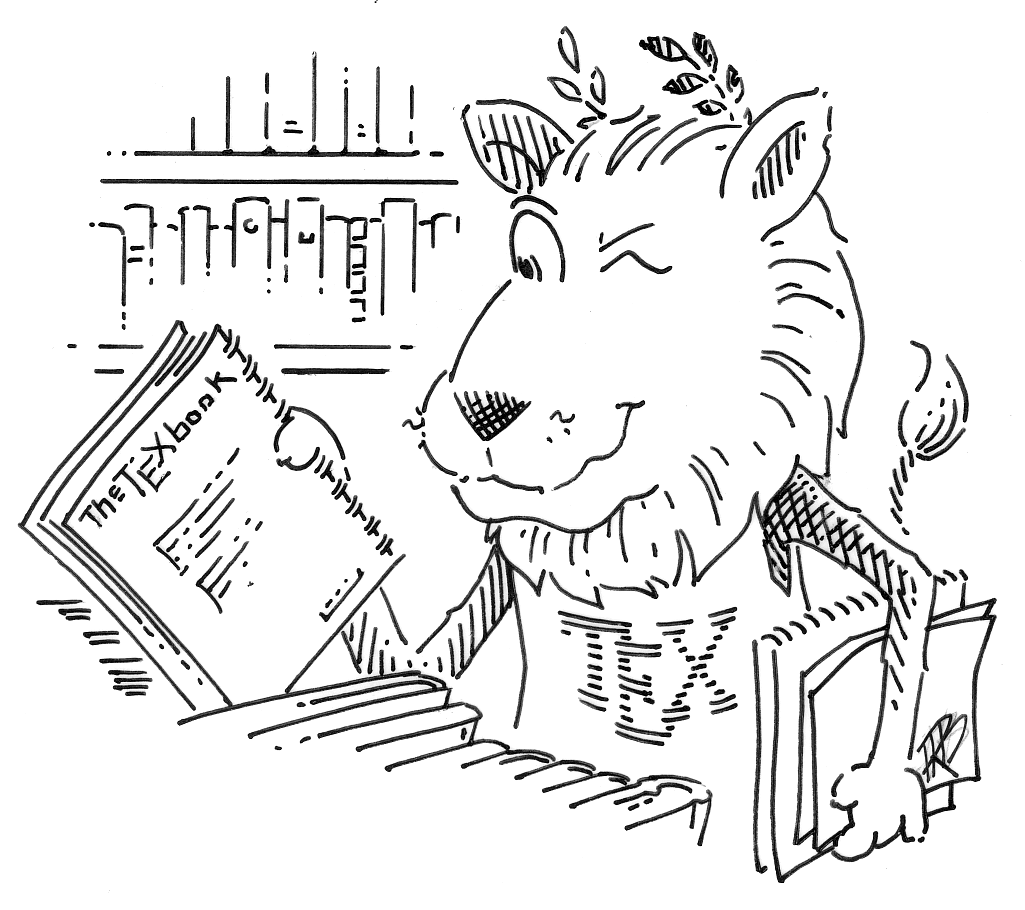
\includegraphics[width=0.35\columnwidth]{image}
	\figcaption{Рисунок збоку від тексту}
	\label{pic1}
\end{wrapfigure}
Вузькі і маленькі рисунки добре виглядають збоку від тексту (рис.~\ref{pic1}), широкі рисунки слід вставляти між абзацами тексту  (рис.~\ref{pic2}).
Зверніть увагу, що при розташуванні рисунка збоку від тексту оточення \texttt{wrapfigure} повинно стояти \emph{перед} потрібним абзацом. Таке оточення підключається за допомогою пакета \href{http://www.ctan.org/pkg/wrapfig}{wrapfig}.

Для розташування на сторінці рисунків і таблиць, які вставляються між абзацами,
\LaTeX{} використовує спеціальний алгоритм, тому такі рисунки і таблиці можуть <<\textit{плавати}>>
по сторінці і виявитись не в тому місці, в якому автор очікує їх побачити.
Це не помилка, а прийняте правило верстки <<\textit{плаваючих}>> об'єктів.

У команді \texttt{\string\includegraphics } імена файлів з рисунками вказуються без розширень (\texttt{.pdf}, \texttt{.png} тощо).

\begin{figure}\centering
	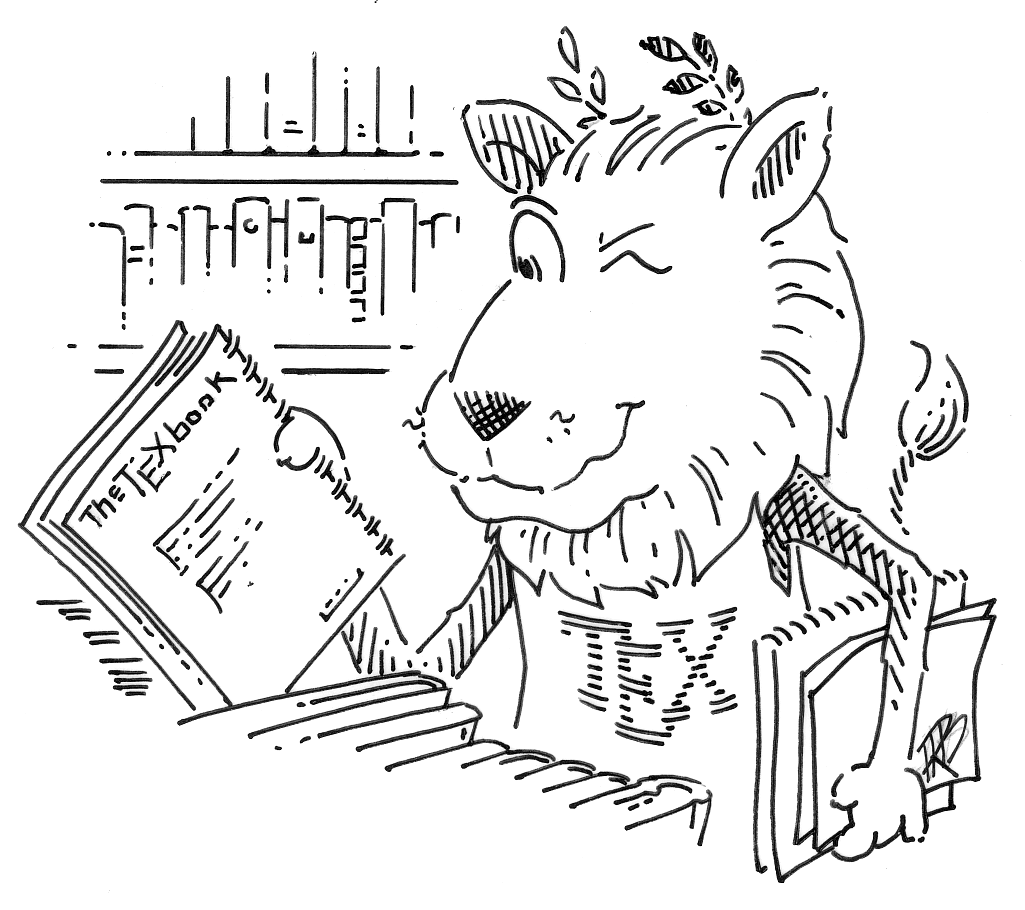
\includegraphics[width=0.9\columnwidth]{image}
	\figcaption{Приклад рисунка між абзацами тексту}
	\label{pic2}
\end{figure}





%%% --------------------------------------------------------
\subsection{Створення графічних об'єктів засобами графічних пакетів}
%%% --------------------------------------------------------





\LaTeX має можливості, які дозволяють створювати графіку прямо в документі. Розглянемо деякі з них.





%%% --------------------------------------------------------
\subsubsection{Створення простих рисунків}
%%% --------------------------------------------------------





Для створення простих рисунків можна використовувати пакет~\href{https://www.ctan.org/pkg/pgf}{TikZ/PGF}, який викликається в преамбулі цього документа як \string\usepackage\{tikz\} (рис.~\ref{pic:tikz}).

\begin{figure}[h!]
	\centering
	\begin{tikzpicture}[scale=1.5]
		\draw[thick, blue]  (-3,0) -- node[ above] {Лінія} (3, 0); % <- рисунок лінії
		\draw[thick, red] (0,0) circle (2); % <- рисунок кола радіуса 2 см
		\draw[thick] (-2,-2) rectangle (2,2); % <- рисунок кола
	\end{tikzpicture}
	\caption{Векторні рисунки, створені графічним пакетом~\href{https://www.ctan.org/pkg/pgf}{TikZ/PGF}}
	\label{pic:tikz}
\end{figure}





%%% --------------------------------------------------------
\subsubsection{Створення діаграм}
%%% --------------------------------------------------------





Для створення схем і діаграм прямо в тексті тез (для тих хто знається) можна використовувати пакет~\href{https://www.ctan.org/pkg/forest}{Forest}.

\begin{figure}[h!]
	\centering
	\begin{forest}
		for tree={%
		l sep=1cm,
		s sep=0.1cm,
		minimum height=0.8cm,
		minimum width=2cm,
		draw %Put lines around each
		}
		[Голова, name= Head, fill=blue!30
		[Лівий, for tree={fill=green!30}  %Format everything below here as children
		[Гілка
		[Гілочка]
		[Гілочка]
		]
		]
		[Правий, for tree={fill=red!30}  %Format everything below here as children
		[Гілка
		[Гілочка]
		[Гілочка]
		]
		]
		]
	\end{forest}
	\figcaption{Діаграма, створена в пакеті~\href{https://www.ctan.org/pkg/forest}{Forest}}
	\label{pic:Forest}
\end{figure}





%%% --------------------------------------------------------
\subsubsection{Побудова графіків}
%%% --------------------------------------------------------





Для побудови графіків за результатами експерименту, використовується пакет~\href{https://www.ctan.org/pkg/pgfplots}{pgfplots}.

\begin{figure}[!h]
	\centering
	\begin{tikzpicture}[trim axis left, trim axis right]
		\begin{axis}[%
				xlabel={$x$, см},
				ylabel={$y$, см},
				width=0.75\linewidth, % Ширина графіка
				scale only axis,
				enlargelimits=false,
				line join=round,
				% === Налаштування сітки ===
				grid = both,
				grid style={line width=.1pt, draw=brown!10},
				major grid style={line width=.2pt,draw=brown!50},
				minor tick num = 4,
			]
			\addplot [color=blue,line width=1pt, mark=*]
			coordinates {%
					(1,   1)
					(2,   4)
					(3,   9)
					(4,   16)
				};
			\addplot [color=red,line width=1pt, mark=triangle*]
			coordinates {%
					(1,   1)
					(2,   10.4)
					(3,   14)
					(4,   15)
				};
			%            \addplot [color=black, domain=1:4] {x^3};
		\end{axis}
	\end{tikzpicture}
	\caption{Графік експериментальних даних, створений в пакеті~~\href{https://www.ctan.org/pkg/pgfplots}{pgfplots}}
	\label{pic:pgfplots}
\end{figure}

Для більш детальної інформації, можна порекомендувати статтю \href{https://habrahabr.ru/post/94931/}{Как делать графики в \LaTeX}, величезний онлайн-ресурс \href{http://www.texample.net/tikz/examples/}{\TeX ample.net}.

Також,  пакет~\href{https://www.ctan.org/pkg/pgfplots}{pgfplots} дозволяє використовувати потужні можливості~\href{http://www.gnuplot.info/}{Gnuplot}~-- програми для побудови та аналізу експериментальних даних.





%%% --------------------------------------------------------
\subsection{Комбінування таблиць і рисунків}
%%% --------------------------------------------------------





Рисунки можна розміщувати в одну колонку (рис.~\ref{subfig1}, \ref{subfig2}), а додавши зірочку <<*>> до оточення \texttt{figure*}, можна їх розташувати так, щоб вони займали дві колонки (рис.~\ref{subfig3}, \ref{subfig4}).

І на рисунки, і на таблиці можна посилатися в тексті, якщо додати позначку \string\label\{<мітка>\} і далі посилатись за допомогою команди \string\ref\{<мітка>\}.

\begin{figure}[t!]
	\centering
	\subcaptionbox{Перший рисунок\label{subfig1}}{%
		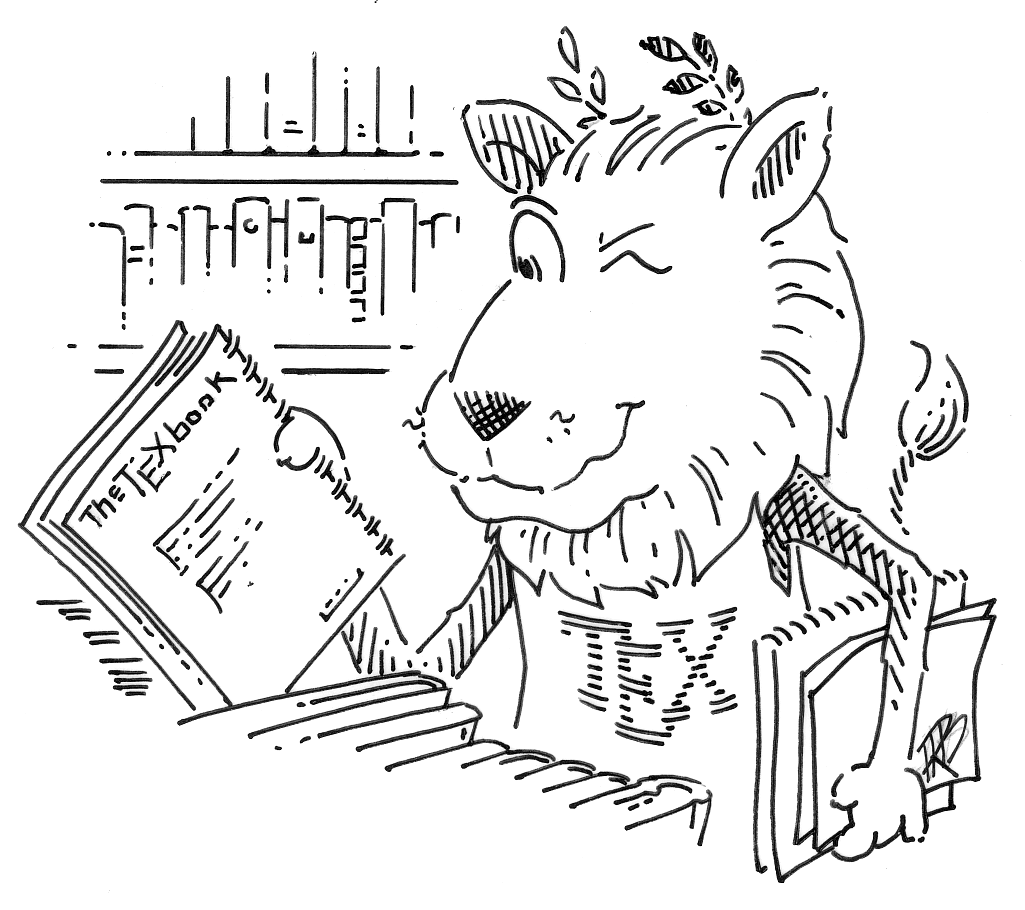
\includegraphics[width=0.95\columnwidth]{image}
	}%
	\\[2ex] % <- для того, щоб рисунки розташувались в колонку
	\subcaptionbox{Другий рисунок\label{subfig2}}{
		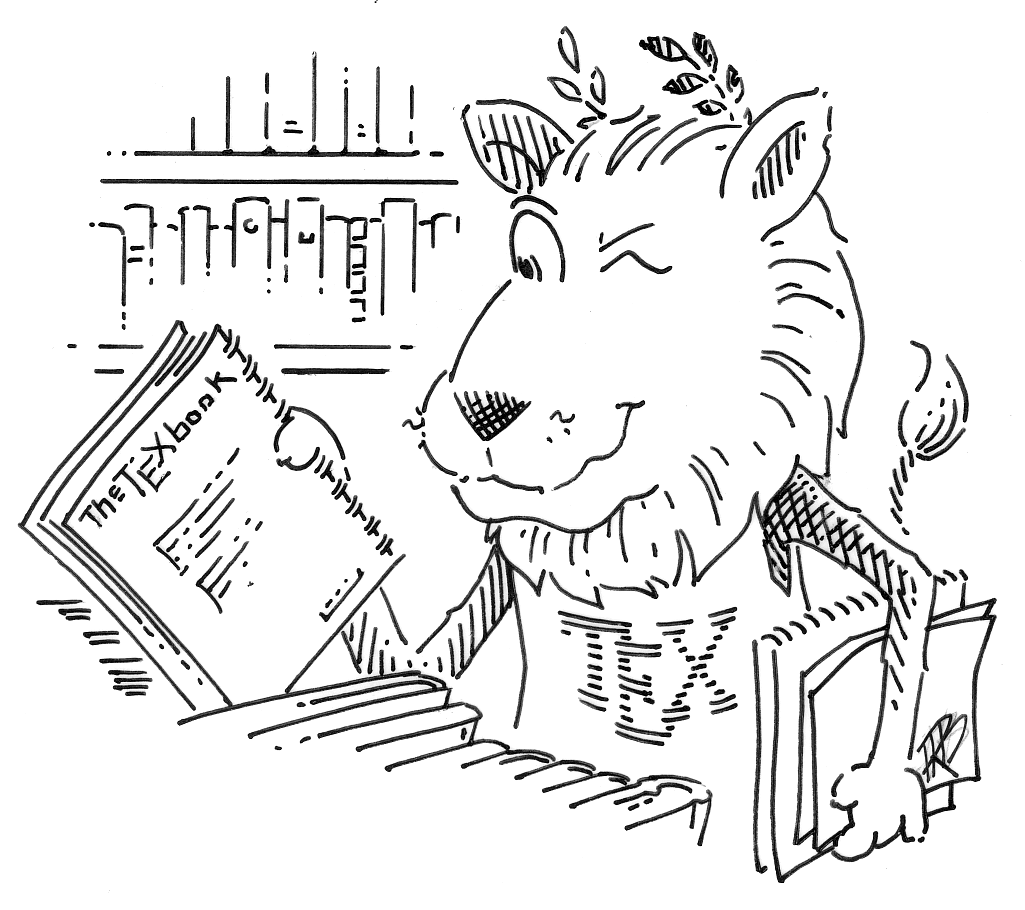
\includegraphics[width=0.95\columnwidth]{image}
	}%
	\figcaption{Рисунки, розташовані поряд}
	\label{Logoipt1}
\end{figure}

\begin{figure*}[h!]
	\centering
	\subcaptionbox{Перший рисунок\label{subfig3}}{%
		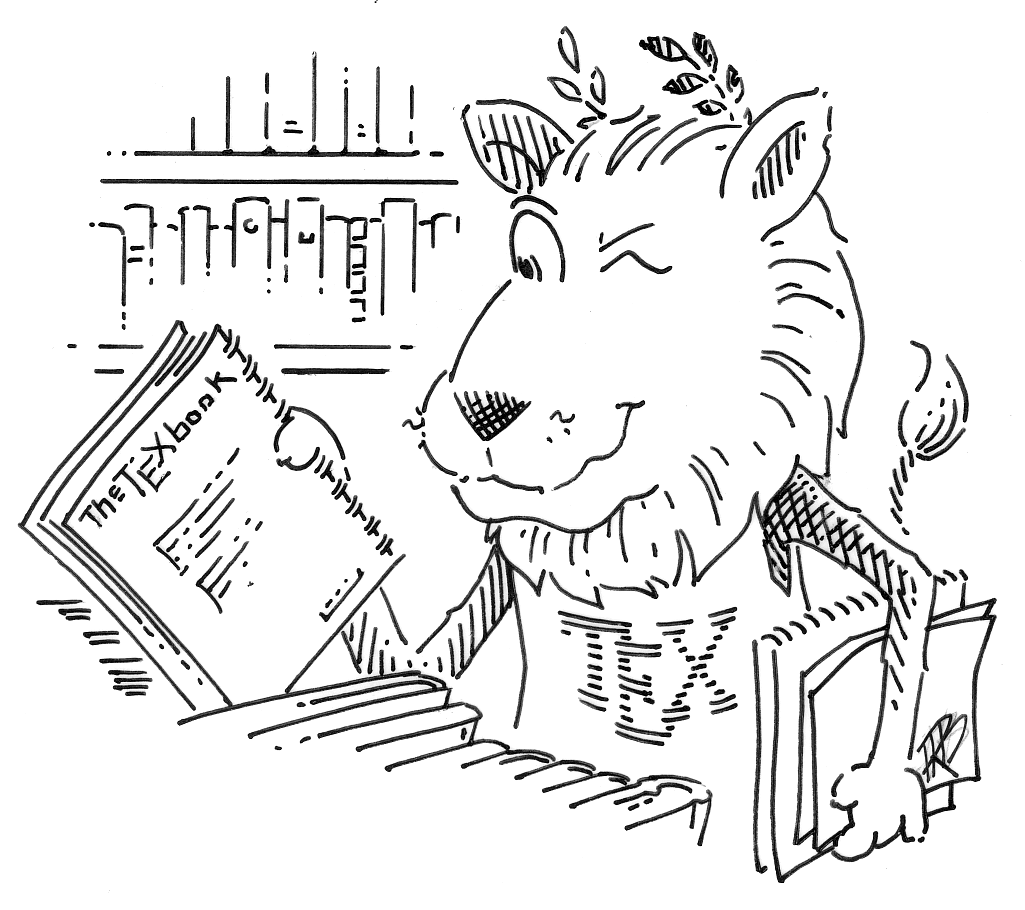
\includegraphics[width=0.95\columnwidth]{image}
	}%
	\qquad %<- для того, між рисунками був проміжок
	\subcaptionbox{Другий рисунок\label{subfig4}}{
		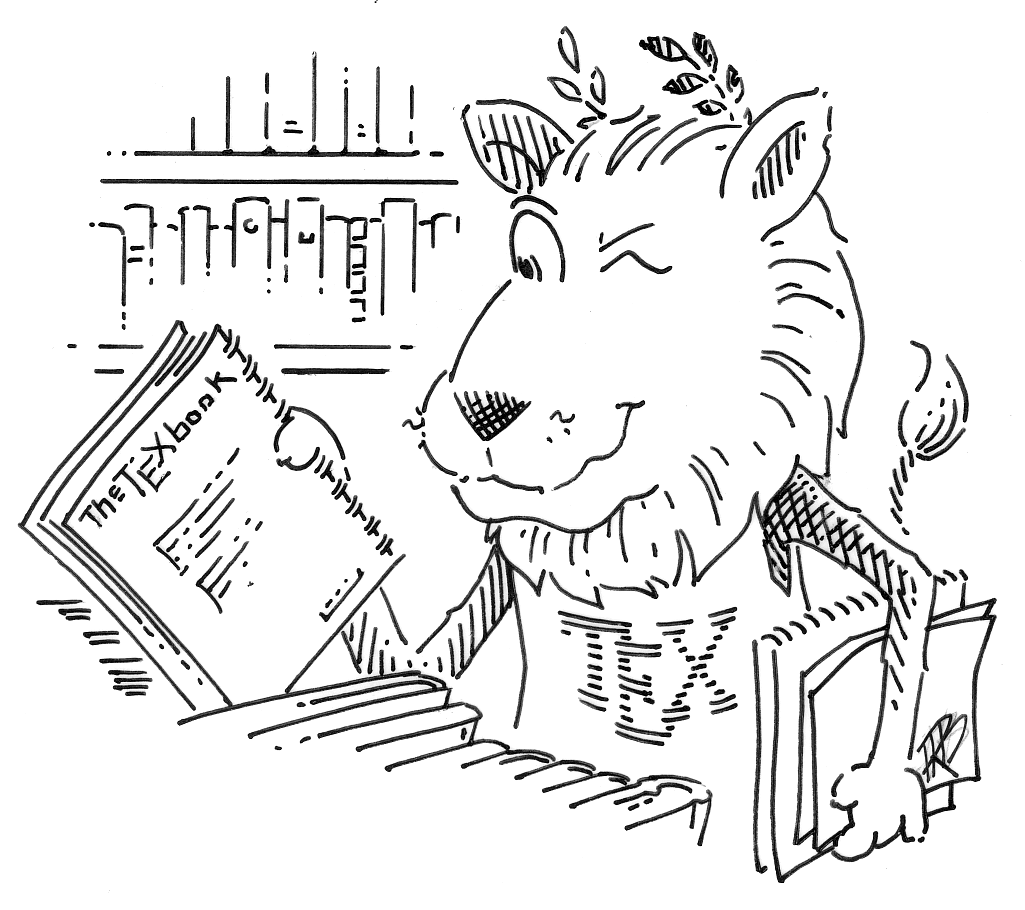
\includegraphics[width=0.95\columnwidth]{image}
	}%
	\figcaption{Рисунки, розташовані поряд}
	\label{Logoipt2}
\end{figure*}





%%% --------------------------------------------------------
\section{Хімічні символи та хімічн формули}
%%% --------------------------------------------------------





Для запису хімічних символів та хімічних формул треба користуватися можливостями пакету \href{https://www.ctan.org/pkg/mhchem}{\texttt{mhchem}}.

Для запису хімічного елемента, треба записувати \string\ce\{Zn\}.

Брутто-хімічну реакції, наприклад таку:
\begin{equation*}
	\ce{CO2 + C ->[k] 2 CO},
\end{equation*}
можна записати за допомогою команди:
\begin{center}
	\string\ce\{CO2 + C ->[k] 2 CO\}
\end{center}

Також зверніть увагу, як треба записувати заголовок статті, якщо в ньому міститься брутто-хімічна формула.
%Ключове слово \string \NoCaseChange\  забезпечить правильне відображення брутто-формули в заголовку.





%%% --------------------------------------------------------
\section{Приклади цитування літератури}
%%% --------------------------------------------------------





На кожне джерело має бути посилання в тексті тез. Приклад оформлення посилань на підручник або книгу~\cite{ZeeGeneralRelativity, Siv1, FLFP}. Якщо посилання йде на конкретну сторінку в книзі, то її слід вказувати таким чином~\cite[стор. 120]{Siv1}.

Посилання на статті в журналі~\cite{Hanson, CookPhysTime, astro-ph/9801252}. Посилання на патент~\cite{patent}. Посилання на online-ресурс~\cite{leinster}.





%%% --------------------------------------------------------
\section{Створення власного \texttt{bib}-файлу}
%%% --------------------------------------------------------





Для оформлення списку літератури, необхідно користуватись власними \texttt{.bib}-файлами. Приклад створення наведено в посиланні \href{https://ctan.math.illinois.edu/macros/latex/contrib/biblatex-contrib/biblatex-gost/doc/biblatex-gost-examples.pdf}{\texttt{Biblatex-GOST examples}}, або в файлі \href{run:author.bib}{\texttt{author.bib}}, який можете знайти в архіві \templateurl.

\texttt{.bib}-Файли -- це файли текстового формату для зберігання списків бібліографічних записів. Кожен запис описує рівно одну публікацію --- статтю, книгу, дисертацію тощо. \texttt{.bib}-Файли можна використовувати для зберігання бібліографічних баз даних. Уважно подивіться на його структуру і заповніть без помилок.

%При створенні цього файлу особливу увагу звертайте на оформлення поля \texttt{author}:

%\begin{tcolorbox}[breakable,enhanced,arc=0mm,colback=gray!5,colframe=red!80!black,leftrule=2mm]
%	\begin{verbatim}
%	author    = {Грайворонський, М. В.
%                  and
%                 Єрещенко, А. А.
%                  and
%                 Монастирський, Г. Є.
%                  and
%                 Гомонай, О. В.},
%\end{verbatim}
%\end{tcolorbox}





%%% --------------------------------------------------------
\section*{Висновки}
%%% --------------------------------------------------------





В цьому розділі узагальнюються головні підсумки роботи. Ви узагальнюєте свої основні результати і факти для читачів. Зазвичай це можна зробити в одному абзаці трьома основними ключовими пунктами і одним переконливим повідомленням того, що читачі повинні усвідомити з Вашої роботи. Це розділ для вираження Ваших думок про можливу майбутню роботу. Спробуйте пояснити своїм читачам, що ще можна зробити. Які подальші кроки, на Вашу думку, можна зробити, які ще питання потребують подальшого дослідження.



\end{document}